\section{Experiment}
\label{experiment}
We start by trying to re-create an observation that Almgren made within the Intrest Rate futures markets.
While looking at the 1 year Eurodollar interest rate futures, he observed that market ``micro-price''
helped predict large price movements in the market.
Specifically he looked at the best bid/ask prices, and the volume weighted average price and observed
that while the market bid/asks didn't move frequently, change of trend in the average price
forecast an impending shift in the market.

Below, we plot the EUR/USD Spot FOREX in an attempt to predict price movement.
%To create a general picture of the order book over time, we took a queue from Almgren's slides on Interest Rate Futures and plot the characteristic prices  of the market.
%That is, we put the top bid, top ask, and volume-weighted average on the same graph and plot these across the timesteps on which the market was open.
%(Henceforth we refer to this as the \emph{bid/ask/avg} graph.)
%We use a volume-weighted average so to put more weight on the high-volume trades, but for this image it makes relatively little difference.
%Sample output for December 3 is given below.

%As a point of note, we apply the Almgren analysis warily.
%Interest Rate Futures, compared to our HFT data, has a relatively large tick size.
%The minimum trade-able unit is significantly larger (perhaps 100 or 1000 times what we see in the HFT) so there are much larger, more observable effects in Almgren's data~\cite{almgren}.
%Still, we hope for some observable change tracking the order book across trades.

\begin{figure}[th]
  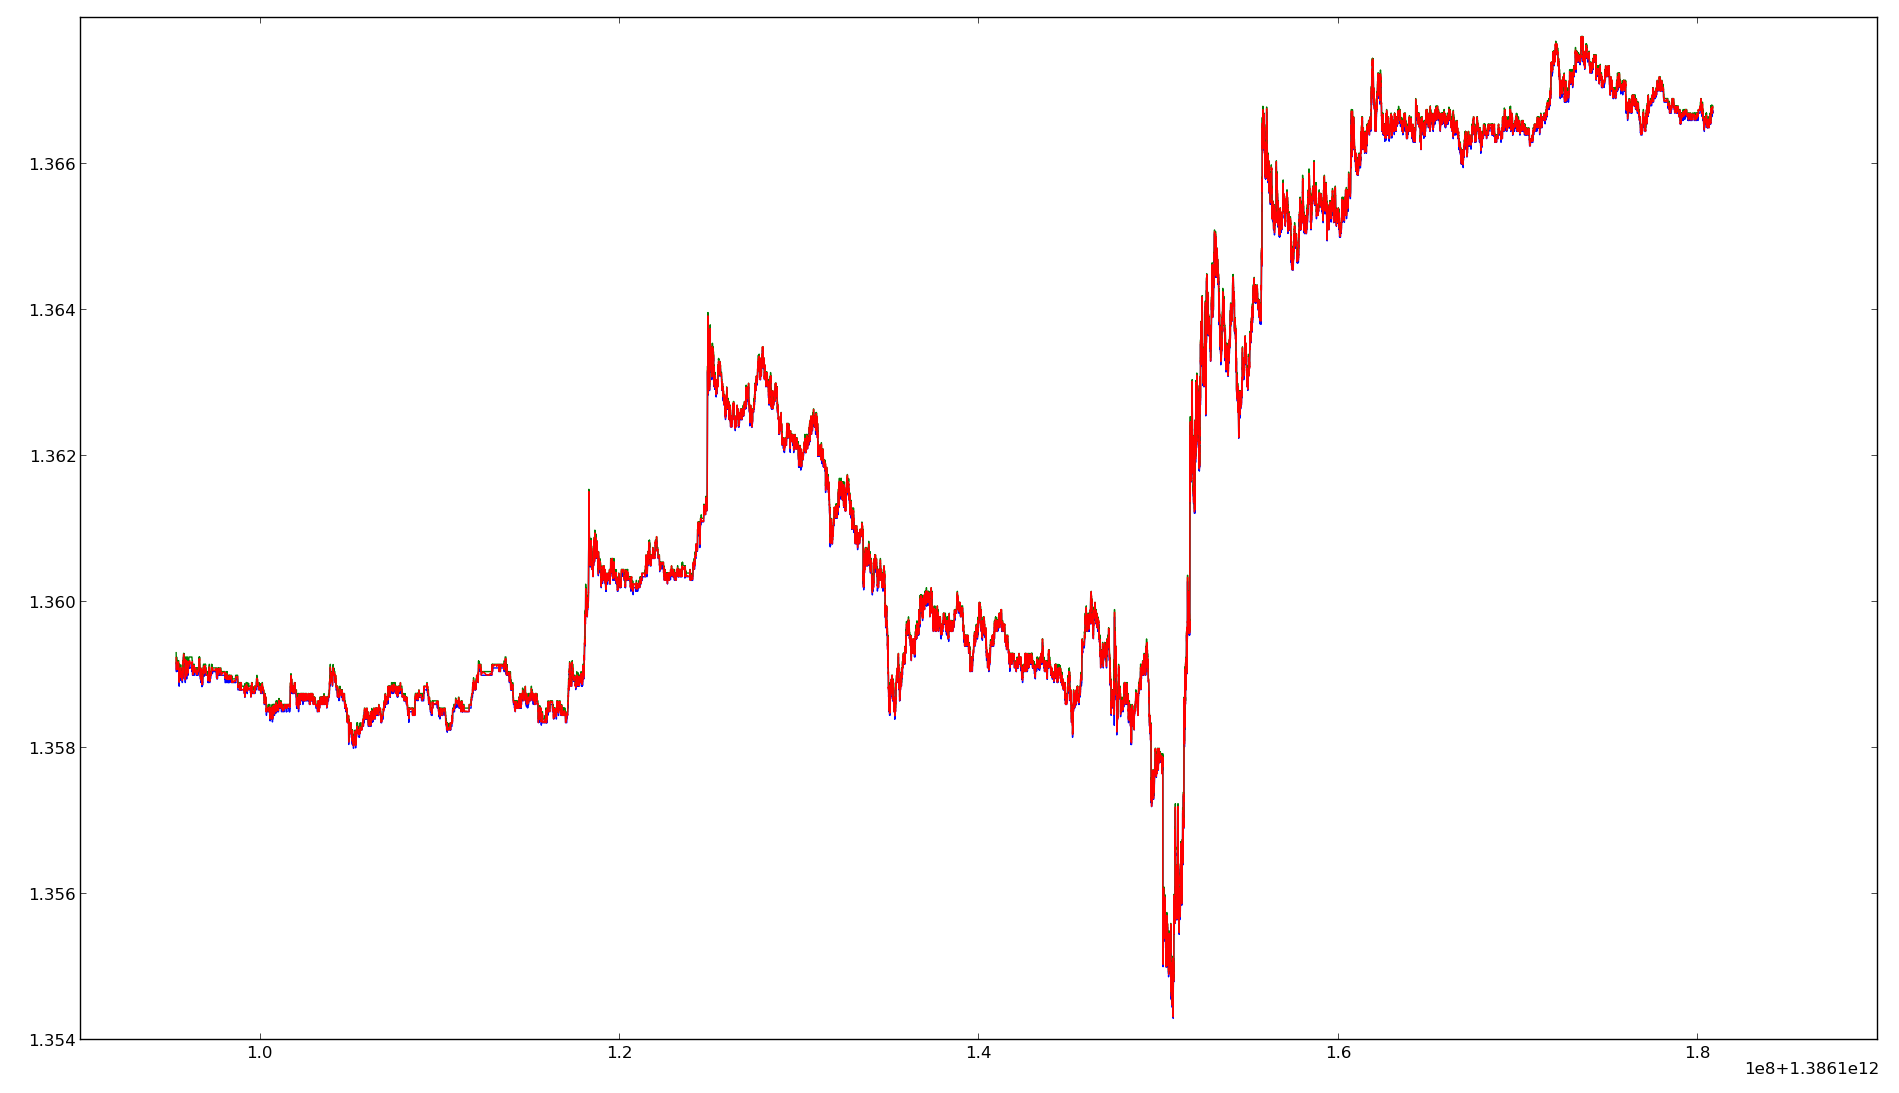
\includegraphics[width=\textwidth]{figures/smoothed_avg_20131204_5.png}
  \caption{Bid, ask, and Volume-weighted price for EUR/USD Spot over 24-hour period. X-axis is time in milliseconds since EPOCH}
  \label{bidaskavg}
\end{figure}

\begin{figure}[th]
  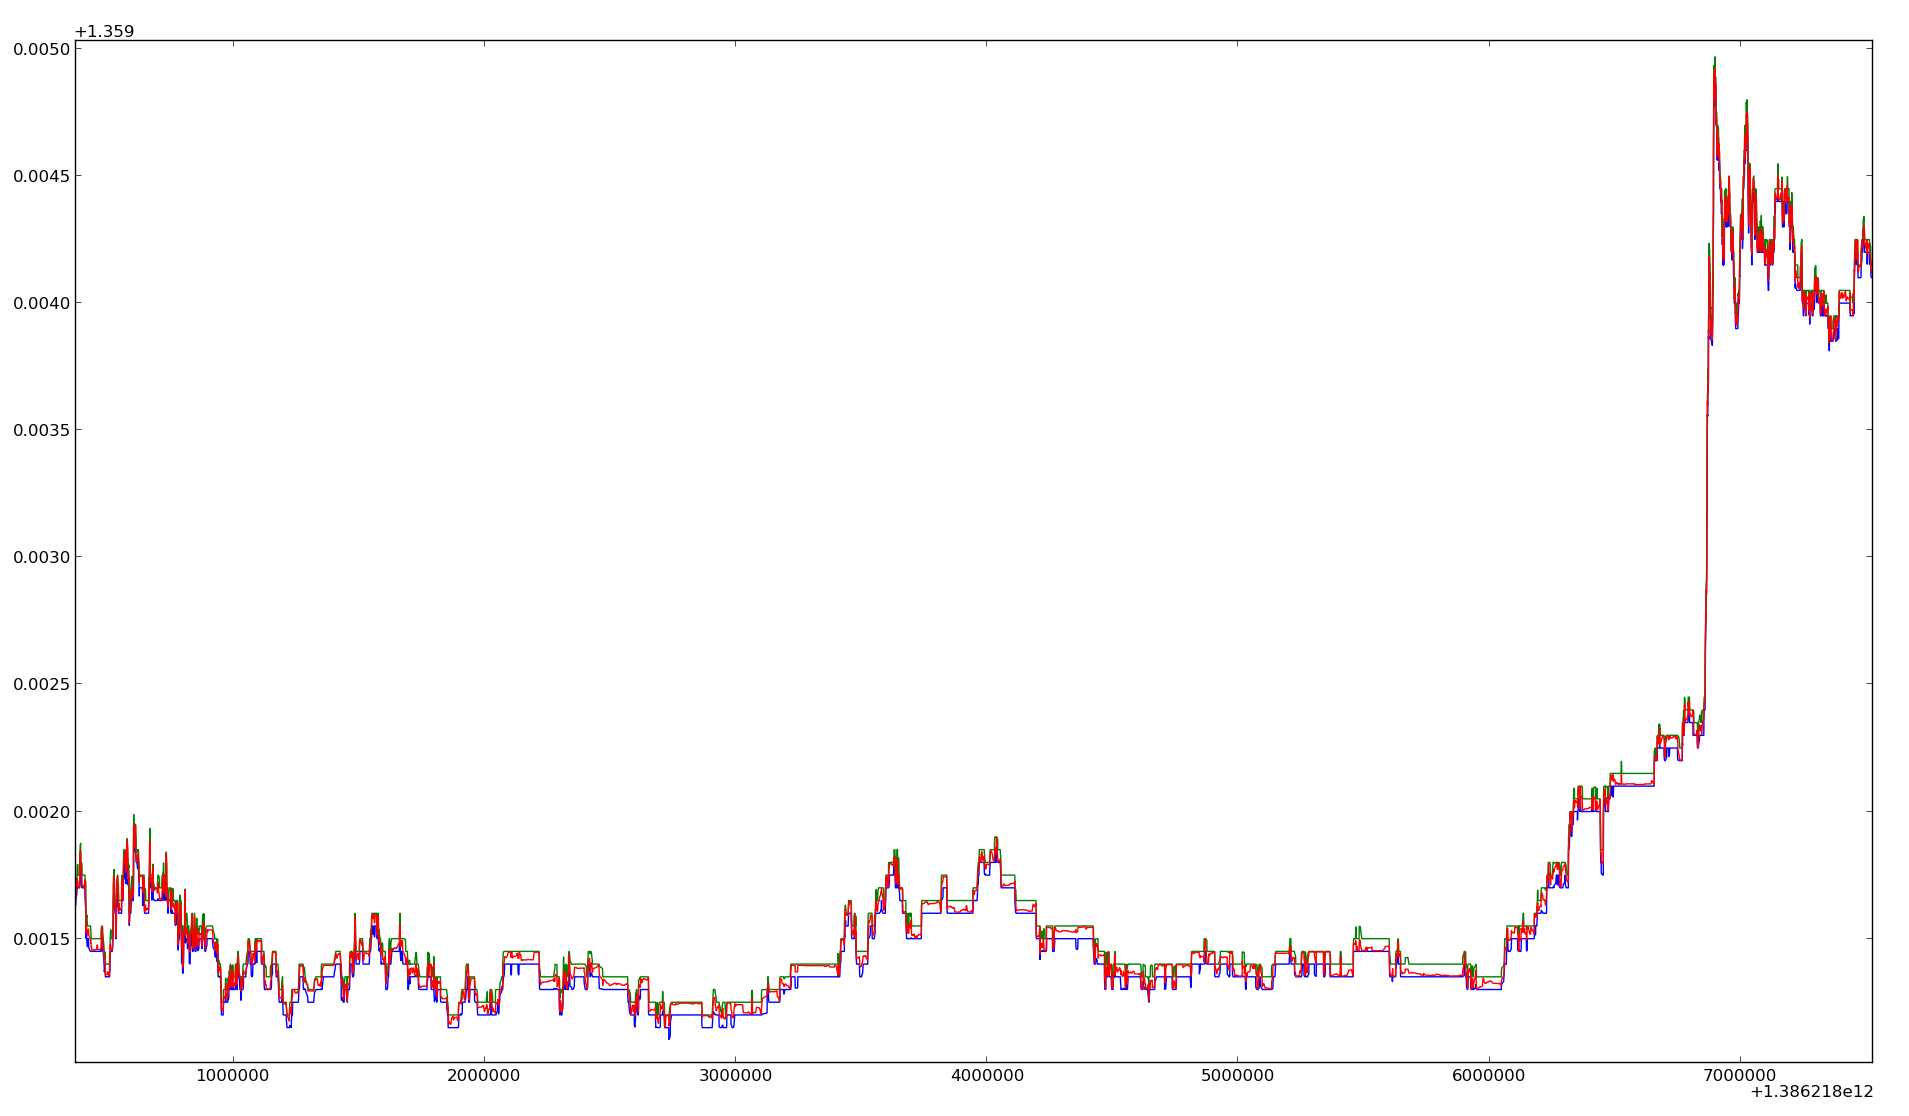
\includegraphics[width=\textwidth]{figures/smoothed_avg_20131204_zoomed.png}
  \caption{Portion of Figure 1, enlarged}
  \label{bidaskavg2}
\end{figure}

Though difficult to read from Figure \ref{bidaskavg}, the blue line is the best bid and the green line is the best ask. 
The red which overpowers the other two is the volume-weighted average.

Figure \ref{bidaskavg2} is an enlargement of the large spike in price in Figure \ref{bidaskavg} preceding the sustained down-trend during the middle of the graph.
Figure \ref{bidaskavg2} shows us that we do not have the nice market micro-structure in the EUR/USD Spot which existed in the Eurodollar interest rates.
Specifically, there is a lot of noise, and small fluctuations in the plot leading up to the large spike in figure two.
This is because the Eurodollar has a large tick size, whereas the EUR/USD does not.
The minimum tradeable unit is significantly larger in the Eurodollar, so prices do not move an entire tick size as frequently.  Our graphs for every other day on which we collected data are similarly difficult to reason about.  They exhibit patterns similar this one; that is, they are often characterized by a sharp rise or fall at one location.
Thus we need a more descriptive picture.

In an attempt to generate a more informative picture and to test our conjecture that trade quantity motivates herding, we plot points of high quantity on top of Figure \ref{bidaskavg}.
The results are in Figure \ref{quantity-deviation}.

\begin{figure}[ht]
  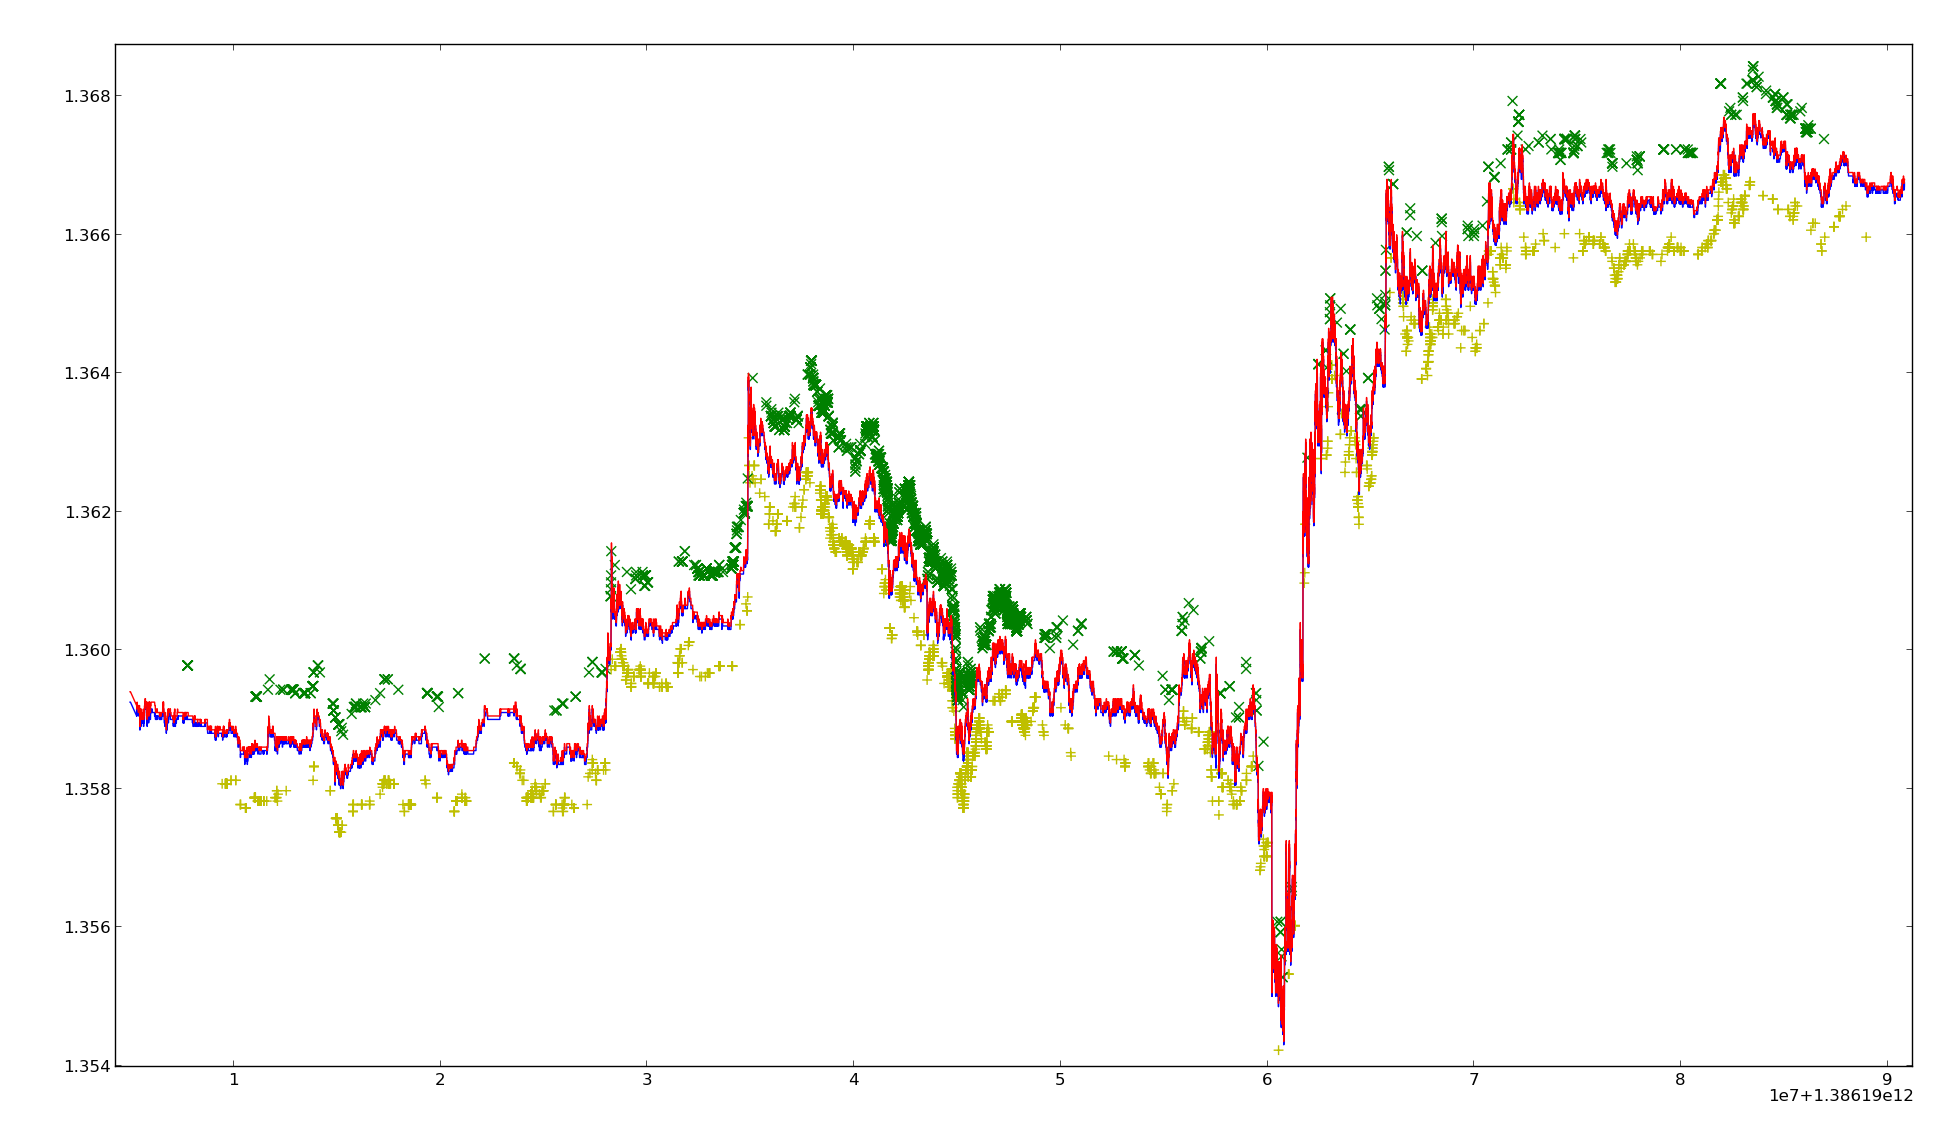
\includegraphics[width=\textwidth]{figures/20131204_quantity_deviation.png}
  \caption{Price along side points indicating two quantities 2 std. dev. from the mean on bid book (Yellow) and ask book (Green).}
  \label{quantity-deviation}
\end{figure}

Points of high quantity are those which the quantity was over 2 standard deviations away from the mean. 
These $(time, price)$ points were then overlaid on the line graph and shifted up or down depending on whether they were for the ask book or the bid book.
In all, there are 9,934 such outlying points, summarized in Figure \ref{quantity-deviation-table}.

\begin{figure}
  \begin{center}
  \begin{tabular}{ r | c c }
    & \textbf{Bid} & \textbf{Ask}\\\hline
    Outliers & 4,525 & 5,409\\
    Average Quantity. & 8,471,857 & 9,656,184 \\
    Std. Deviation & 6,196,046 & 6,432,082 \\
  \end{tabular}
  \end{center}
  \caption{Statistics on outliers from Figure \ref{quantity-deviation}}
  \label{quantity-deviation-table}
\end{figure}

%% The average 
%% ; 4,525 are bids and 5,409 are asks.
%% FIgure metadata
%% There were 4525 outliers on the bids, and 5409 outliers on the asks...
%% All of them were positive outliers, no negative outliers..
%% Average bid qty is: 8,871,857 std. dev. is: 6,196,046 (Thats a high std. dev ~70% of mean)
%% Num of pos bid qty outliers are 4525
%% Num of neg bid qty outliers are 0
%% Average ask qty is 9,656,184, std. dev. is: 6,196,046
%% Num of pos ask qty outliers are 5409
%% Num of neg ask qty outliers are 0

%% TODO delete table?

Before analyzing the shifts and trends in this graph, we step back and review the premises for our model.
Trading is happening in a high-frequency setting where informed traders, uniformed traders, and liquidity providers interact. 
We focus on the behavior of the HFT liquidity provider\textemdash these are the algorithms that are profiting through high-quantity, low-prices trades that happen at very high frequency.
These liquidity providers do best in a fair, stable market, where drastic price shifts are rare.
As such, they must continuously monitor their competitors (the informed traders) to guard themselves against private information within the market. 
If a trader gains a large information advantage, the liquidity provider is liable to suffer.
Therefore providers use some metric like the VPIN to monitor the market and identify when to withdraw.

On to the graph, we discuss it in terms of three segments.
Segment 1 begins at time 0 and continues until time 3.5.
Segment 2 begins at time 3.5 and continues until time 4.5.
Segment 3 begins at time 4.5 and continues until time 6.
Segment 4 is the large spike we see from time 6 until time 6.5, and lastly Segment 5 begins at time 6.5 and continues until the end.

Throughout this discussion, we refer to outlying price points and liquidity providers interchangeably.
This is because liquidity providers are the players who are making these markets\textemdash the support behind the large bid and ask quantities that define the outliers.

At the beginning, in Segment 1, we see that the prices are relatively stable. 
Prices fluctuate and even jump at one point, but the overall trend is a flat line. 
Accordingly, liquidity providers are active in the market as evidenced by the fair number of outlying points on both the bid and ask side of the bid/ask line. 

This trend continues until we reach the downturn at Segment 2.
Here we have a large density of outliers on both sides of the graph, indicating that liquidity providers are making offers in an attempt to stabilize prices. 
On the ask side we see the greatest density, which makes sense because the price is dropping and sellers prefer a higher price. 
The liquidity providers are losing money throughout Segment 2 as they fight an apparently unstoppable price trend.
From our perspective as observers, we can look at this downtrend and hypothesize that a group of informed traders has some information advantage that is predicting the future prices for them. 
Liquidity providers have no such ability to see the future, and so they monitor the price history and plan their next move. 
After the small spike in the middle of this segment, we see liquidity providers leave the market.

Their VPIN signal (or similar indicator) flagged the market as too dangerous to remain in\textemdash the likelihood that informed traders are making decisions has risen significantly.
The signal produces this flag because it sees that the volume clock is out of sync with the price clock, which supports our hypothesis that volume plays a role in herding behavior.
Unfortunately we cannot use this rule to predict herding as we had hoped, nevertheless it helps us identify herd behavior as it happens.

Returning to the graph, we see liquidity providers continue to leave the market throughout Segment 3.
By the time we exit Segment 3, there is very little liquidity within the market; there is hardly any support for prices on the bid and ask sides.
Hence movements in both directions are quick and exaggerated. 
This accounts for the spike we see in Segment 4. 
Without liquidity providers to support it, the market swings out of control momentarily.
Finally, in Segment 5 the market stabilizes and liquidity providers return, yielding a pattern similar to what we saw in Segment 1.

Our initial objective was to predict herding behavior through careful monitoring of volume. 
We hypothesized that volume was an important contributor to herding.
Unfortunately, our findings do not support this claim.
That said, although quantity is not a predictive indicator, it does work as an on-line indicator for price shifts.
Using the VPIN model, we can predict that liquidity provision will decrease after a herd-like event.
This is exactly what we saw in Segment 3 of Figure \ref{quantity-deviation}

As a result of the decrease in liquidity provision, we conclude that future price movements will be drastically over-exaggerated until the HFTs return to the market and start providing liquidity again.
While it is difficult to predict the direction of this movement, we can nevertheless find a profitable trading strategy based on trading a derivative of the security (e.g. an option on the EUR/USD Spot FX) we are observing which will increase in price due to increase in volatility.

\subsection{Prefix Tree}
Unsatisfied by our initial attempt at characterizing herd behavior, we decided to take a different approach at identifying parameters that would predict price changes.
Instead of working from our intuition or experience, which had thus far been insufficient at describing algorithms (or at least at describing the data available to us) we decided to apply machine learning techniques to identify parameters of interest.
Our goal was to say something meaningful about trends in the bid and ask prices.
To this end, we constructed a simple prefix tree modelling price patterns.

The prefix tree was constructed as follows. 
First, we extracted from the order book the state of the top bid and top ask at each point in time.
Ignoring quantity and caring only for the price point, we stepped through the data and marked a $A$, 0, or $B$ if the price had raised, stayed the same, or fallen since the previous timestep.
This left us with a long string of prefix information.
We then iterated over this string, constructing a tree of each newly encountered prefix. 
This process is best explained with an example. 

Given the string $\{ A, A, A, 0, B, A, A, B\}$, we begin with a tree consisting of only the root and consider the first element.
Reading an $A$, we construct a new node labeled ``A'' and having count 1 and place a directed edge from the root to this node.
This means we have found a new prefix.
Having created a new node, we return to the root.
Reading the next element, an $A$, we follow the edge to the node labeled ``A'' that we just created and increment its count to 2. 
This means we have followed an old prefix. 
Next we consider the third sequence element, $A$, and construct a new node labeled ``A'' and having count 1 as a child of the current node.
Jumping back to the root because we just created a new node, the next two sequence elements result in the children ``0'' and ``B'' being added to the root.
The last three elements represent one new sequence, which we reach by traveling from root to ``A'', incrementing the count to 3, from ``A'' to the next node labeled ``A'', incrementing its count to 2, and finally creating a new node ``B'' as a child of this node.
Figure \ref{prefix-example} shows the entire tree created following the above sequence.

\begin{figure}
  \begin{center}
  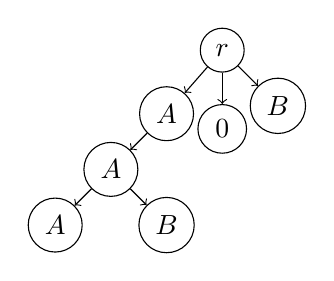
\begin{tikzpicture}
    \node [draw,circle] (1) {$r$};
    \node [draw,circle,below left of=1,yshift=-.1cm] (2) {$A$};
    \node [draw,circle,below left of=2] (3) {$A$};
    \node [draw,circle,below left of=3] (4) {$A$};
    \node [draw,circle,below right of=3] (5) {$B$};
    
    \node[draw,circle,below of=1] (6) {$0$};
    \node[draw,circle,below right of=1] (7) {$B$};

    \draw[->] (1) -- (2);
    \draw[->] (1) -- (6);
    \draw[->] (1) -- (7);
    \draw[->] (2) -- (3);
    \draw[->] (3) -- (4);
    \draw[->] (3) -- (5);

  \end{tikzpicture}
  \end{center}
  \caption{Example prefix tree, constructed from sequence  $\{ A, A, A, 0, B, A, A, B\}$}
  \label{prefix-example}
\end{figure}


In the presence of herding, we would expect to see a strong price trend and thus an unbalanced tree.
The paths present in the final tree give the space of all encountered prefixes, which will be skewed left or right if herding occurs.
Additionally the counts, which give the probability of moving the a node to any one of its children, should be skewed if herding occurred.

Our first attempt in constructing a prefix tree over an entire week's worth of data gave us a structure with a huge proportion of zeros.
Almost 90\% of the sequence elements were zeros, leading to a tree with a disproportionately high number of paths made almost exclusively of zeros.
Figure \ref{prefix-tree-stats} summarizes this data by giving the probability of choosing a zero from any node in the graph.
To generate the plot we simply examined the at most 3 children of each node and compared the probabilities of advancing to each.

At any rate, the tree full of zeros had no use to us as a prediction mechanism. 
We could not say anything meaningful about price trends if the vast majority of events led to no change at all.
But looking back, finding this many zeros in the tree was not unexpected.
We knew ahead of time that the order book changed in small ways between timesteps, and that many of these did not affect the best bid/ask.
For instance any simple transaction between one of the other, non-top securities would lead to two order book changes (one documenting the buyer, the other documenting the seller) neither of which affected the top row.
So we decided to prune the prefix string, omitting all the zero entries.

With this new, pruned input string containing only the directions $A$ and $B$ that the order book shifted between rounds, we expected to see a much more insightful predictor of prices.
Having filtered the inconclusive data, asymmetries within the tree would now become apparent, even over-characterized.
Yet our findings were decidely null.

\begin{figure}[t]
  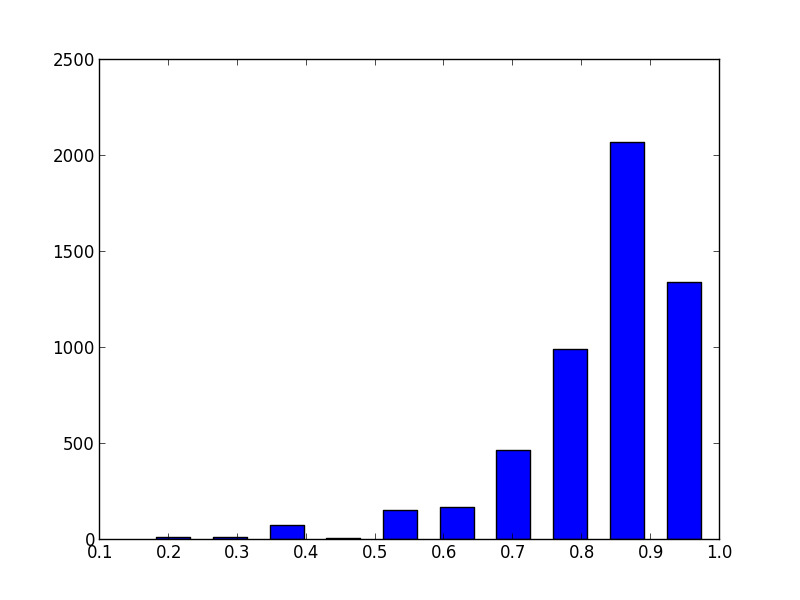
\includegraphics[width=0.5\textwidth]{figures/tree-prob-all-unfiltered.png}
  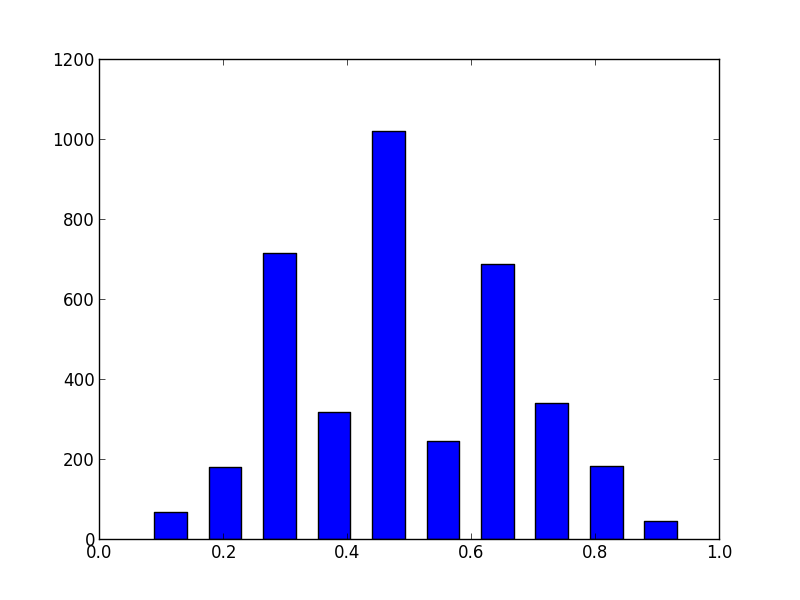
\includegraphics[width=0.5\textwidth]{figures/tree-prob-all-filtered.png}
  \caption{Prefix tree findings: the left is the probability of choosing 0 from a given node in the unpruned tree. The right is the probability of choosing $A$ in the pruned tree.}
  \label{prefix-tree-stats}
\end{figure}


The second plot in Figure \ref{prefix-tree-stats} shows the probability of choosing $A$ from any node in the tree.
It follows a perfectly normal distribution, indicating one of two things.
Either there was no herding throughout the week or our data failed to capture any interesting characteristics of the market.
We fear it was the latter.

%% NOTES ON TAPESTRY
%% we may be looking at data in the wrong dimension. If we can fit a curve from a higher 
%% dimension to it, we may have a line
%% Feature vector shoudl be deviation from mean volume

%% SVM 


%% Fig2 meta
%% Average bid qty is: 8871857.65038, std. dev. is: 6196046.22068
%% Num of pos bid qty outliers are 10
%% Num of neg bid qty outliers are 0
%% Average ask qty is 9656184.66183, std. dev. is: 6196046.22068
%% Num of pos ask qty outliers are 2
%% Num of neg ask qty outliers are 0
%% 3 only gives me 12 pts.
